% STATUS: ACTIVE | DERIVATION (2026-09-16, coordinate revised 2026-09-18): the z-axis motion gain a_z(h_bar) of the
%   plane wall (a_nom / c_perp, c_perp from model/wall_effect/calc_correction_functions.m) written as a function of
%   w_bar - w_bar_s, where w_bar_s is the WALL SURFACE position in the particle-centre coordinate w_bar (plane: 0),
%   so w_bar - w_bar_s = h_bar (centre to surface, contact at 1). The 2026-09-16 version put w_bar_s at the contact
%   height (plane: 1) and used the surface gap w_bar - w_bar_s = h_bar - 1; the two are the same law with every
%   constant shifted by one radius (old c_0 = new c_0 + 1, old d_1 = new d_1 + 1; verified bit-identical in closed loop).
%   Figures: plot_abar_vs_gap.m, probe_fig11_s_from_fit.m, probe_plane_pade.m, probe_cell_pade.m (test_script/scratch).
%   Equations only.
% Compile: xelatex 0916_abar_gap_polynomial.tex

\documentclass[11pt,a4paper,fontset=none]{ctexart}
\usepackage[fleqn]{amsmath}
\usepackage{amssymb,bm}
\setlength{\mathindent}{0pt}
\usepackage{graphicx}
\usepackage{pdflscape}
\usepackage{geometry}
\geometry{margin=2.0cm}

\setlength{\parindent}{0pt}
\setlength{\parskip}{0.80em}
\linespread{1.08}
\setlength{\abovedisplayskip}{10pt}
\setlength{\belowdisplayskip}{10pt}

\newcommand{\ba}{\bar{a}}
\newcommand{\bw}{\bar{w}}
\newcommand{\bh}{\bar{h}}
\newcommand{\gs}{(\bw - \bw_s)}

\begin{document}

\section{$a_z(\bh)$ from the plane $c_\perp$}

(bars denote lengths divided by $R$: $\bh := h/R$, sphere centre to wall surface, contact at $\bh = 1$;
$a_{\mathrm{nom}} := \Delta t/\gamma_N$ [$\mu$m/pN]; $\ba_z := a_z/a_{\mathrm{nom}}$)

\begin{align*}
c_\perp(\bh)
  &= \frac{1}{\;1 - \dfrac{9}{8}\,\dfrac{1}{\bh}
       + \dfrac{1}{2}\,\dfrac{1}{\bh^{3}}
       - \dfrac{57}{100}\,\dfrac{1}{\bh^{4}}
       + \dfrac{1}{5}\,\dfrac{1}{\bh^{5}}
       + \dfrac{7}{200}\,\dfrac{1}{\bh^{11}}
       - \dfrac{1}{25}\,\dfrac{1}{\bh^{12}}\;} \\[4pt]
a_z(\bh)
  &= \frac{a_{\mathrm{nom}}}{c_\perp(\bh)} \\[4pt]
\ba_z(\bh)
  &= 1 - \frac{9}{8}\,\frac{1}{\bh}
       + \frac{1}{2}\,\frac{1}{\bh^{3}}
       - \frac{57}{100}\,\frac{1}{\bh^{4}}
       + \frac{1}{5}\,\frac{1}{\bh^{5}}
       + \frac{7}{200}\,\frac{1}{\bh^{11}}
       - \frac{1}{25}\,\frac{1}{\bh^{12}} \\[4pt]
\ba_z(1) &= 0, \qquad \frac{d\ba_z}{d\bh}\Big|_{1} = 1, \qquad
\lim_{\bh\to\infty} \bh\,\bigl(1 - \ba_z\bigr) = \frac{9}{8}
\end{align*}

\section{Height coordinate and the wall surface}

($\bw := w/R$, particle centre along the wall normal; $\bw_s$ = position of the wall surface on the same axis, known;
the plane's surface is the origin of $\bh$, so $\bw_s = 0$ there)

\begin{align*}
\bh          &= \bw - \bw_s \\
\text{contact:}\qquad \bw - \bw_s &= 1 \\
\text{band used:}\qquad \bw - \bw_s &\ge 1.1
\end{align*}

\section{$a_z$ as a function of $\bw - \bw_s$}

\begin{align*}
\ba_z\gs
   &= 1 - \frac{9}{8}\,\frac{1}{\gs}
       + \frac{1}{2}\,\frac{1}{\gs^{3}}
       - \frac{57}{100}\,\frac{1}{\gs^{4}} \\
&\qquad
       + \frac{1}{5}\,\frac{1}{\gs^{5}}
       + \frac{7}{200}\,\frac{1}{\gs^{11}}
       - \frac{1}{25}\,\frac{1}{\gs^{12}}
\end{align*}

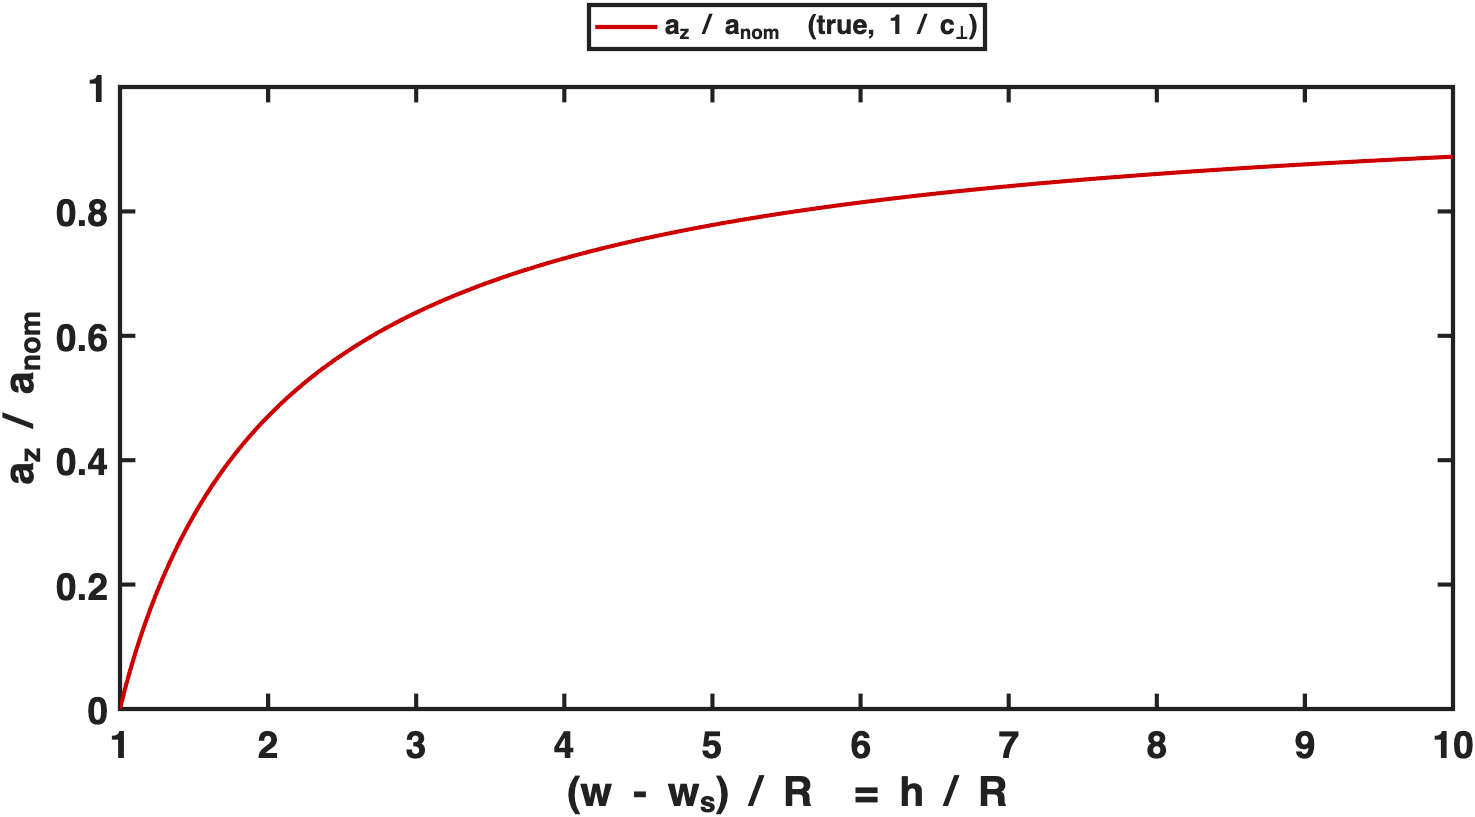
\includegraphics[width=\textwidth]{figures/abar_vs_gap.png}

\section{$a_z$ with the surface gap scaled by $s$}

($s$ scales the gap $\gs - 1$ between the sphere surface and the wall; $s = 1$ is the plane)

\begin{align*}
\ba_z\gs
   &= 1 - \frac{9}{8}\,\frac{1}{1 + s\,\bigl(\gs - 1\bigr)}
       + \frac{1}{2}\,\frac{1}{\bigl(1 + s\,(\gs - 1)\bigr)^{3}} \\
&\qquad
       - \frac{57}{100}\,\frac{1}{\bigl(1 + s\,(\gs - 1)\bigr)^{4}}
       + \frac{1}{5}\,\frac{1}{\bigl(1 + s\,(\gs - 1)\bigr)^{5}} \\
&\qquad
       + \frac{7}{200}\,\frac{1}{\bigl(1 + s\,(\gs - 1)\bigr)^{11}}
       - \frac{1}{25}\,\frac{1}{\bigl(1 + s\,(\gs - 1)\bigr)^{12}}
\end{align*}

($\delta$ shifts the effective wall below the reference surface; $\delta = 0$ is the plane; band $1.1 \le \bw - \bw_s \le 5.5$,
least squares on the Fig.\ 11 curves, probe\_plane\_offset\_law.m)

\begin{align*}
\ba_z\gs &= D_\perp\!\Bigl(\frac{1}{\gs + \delta}\Bigr) \\
\ba_z\gs &= D_\perp\!\Bigl(\frac{1}{1 + s\,\bigl(\gs + \delta - 1\bigr)}\Bigr) \\[4pt]
\text{plane:}\quad \delta &= -0.001 \quad (\text{rms } 0.0016) \\
\text{cell:}\quad  \delta &= +1.050 \quad (\text{rms } 0.0061,\ 2.6\%;\ \text{with } s \text{ free: } \delta = 1.042,\ s = 1.004) \\
\text{sphere:}\quad \delta &= -0.039,\ s = 1.323 \quad (\text{rms } 0.0055,\ 20\%;\ \delta \text{ alone: rms } 0.040)
\end{align*}

\begin{landscape}
\vspace*{\fill}
\noindent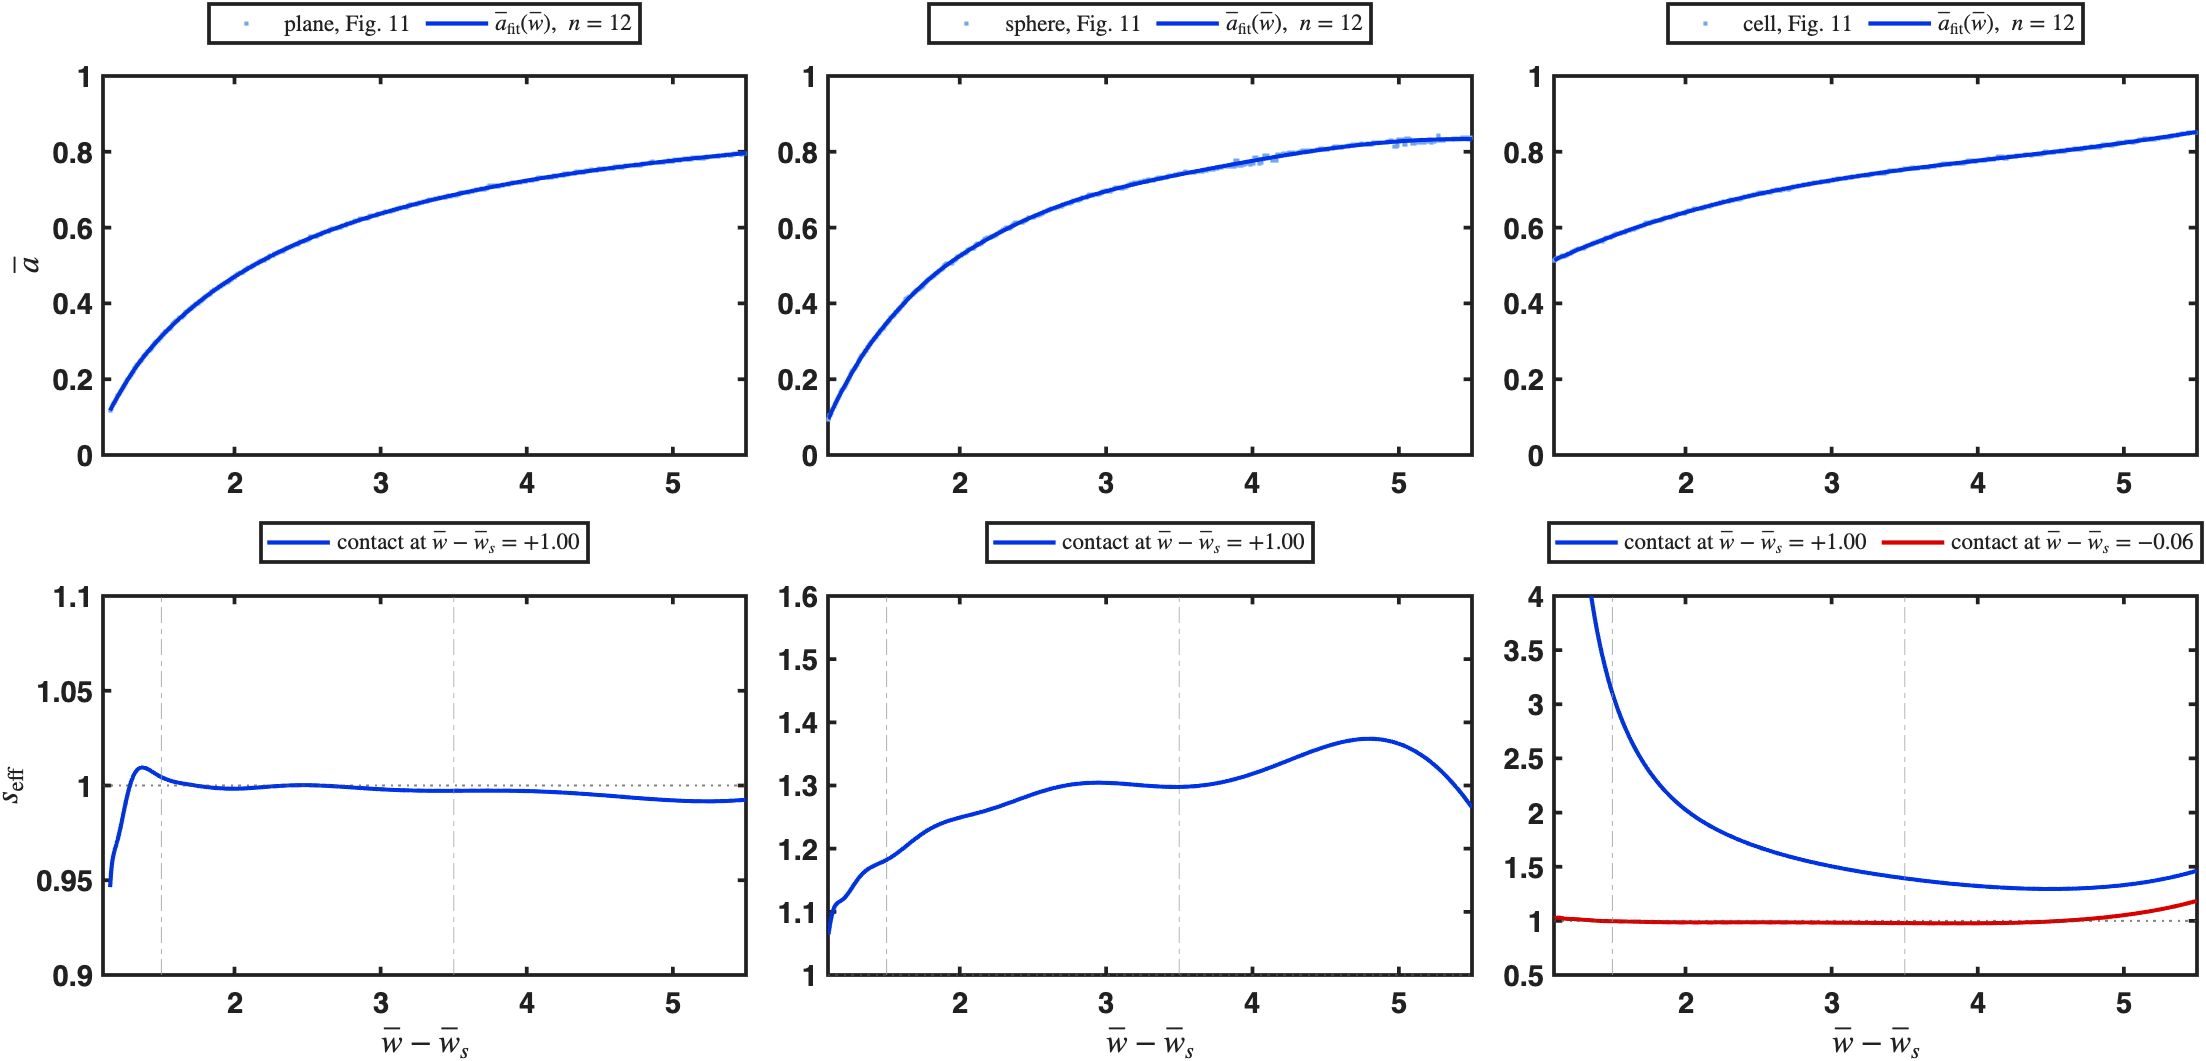
\includegraphics[width=\linewidth]{figures/fig11_s_from_fit.png}
\vspace*{\fill}
\end{landscape}

\section{Two-point Pad\'e form of $\ba_z\gs$}

($\ba_z(\infty) = 1$ built in; the two ends are the contact $\bw - \bw_s = 1$ and the far field)

\begin{align*}
\ba_z\gs
  &= \frac{\gs^{2} + c_1\,\gs + c_0}
          {\gs^{2} + d_1\,\gs + d_2} \\[6pt]
\ba_z(1) &= \frac{1 + c_1 + c_0}{1 + d_1 + d_2} \\
\frac{d\ba_z}{d\gs}\Big|_{1} &= \frac{(2 + c_1)(1 + d_1 + d_2) - (1 + c_1 + c_0)(2 + d_1)}{(1 + d_1 + d_2)^{2}} \\
\lim_{\bw - \bw_s \to \infty} \gs\,\bigl(1 - \ba_z\bigr) &= d_1 - c_1
\end{align*}

\begin{align*}
[1/1],\ c_1 = d_2 = 0:\qquad
\ba_z\gs &= \frac{\gs + c_0}{\gs + d_1} \\
\ba_z(1) &= \frac{1 + c_0}{1 + d_1} \\
\frac{d\ba_z}{d\gs}\Big|_{1} &= \frac{d_1 - c_0}{(1 + d_1)^{2}} \\
\lim_{\bw - \bw_s \to \infty} \gs\,(1 - \ba_z) &= d_1 - c_0 \\[6pt]
\text{plane},\ \ba_z(1) = 0 \ \Rightarrow\ c_0 = -1:\qquad
\ba_z\gs &= \frac{\gs - 1}{\gs + d_1} \\
d_1 &= 0 \ \ \text{(slope 1)}\qquad \text{or}\qquad d_1 = \frac{1}{8} \ \ \text{(far } \tfrac{9}{8}\text{)} \\[6pt]
[2/2],\ \text{plane (slope 1, curvature } -\tfrac{327}{200}\text{, far } \tfrac{9}{8}\text{)}:\qquad
c_0 &= \frac{102}{127}, \quad c_1 = -\frac{229}{127}, \quad d_1 = -\frac{689}{1016}, \quad d_2 = -\frac{1}{8}
\end{align*}

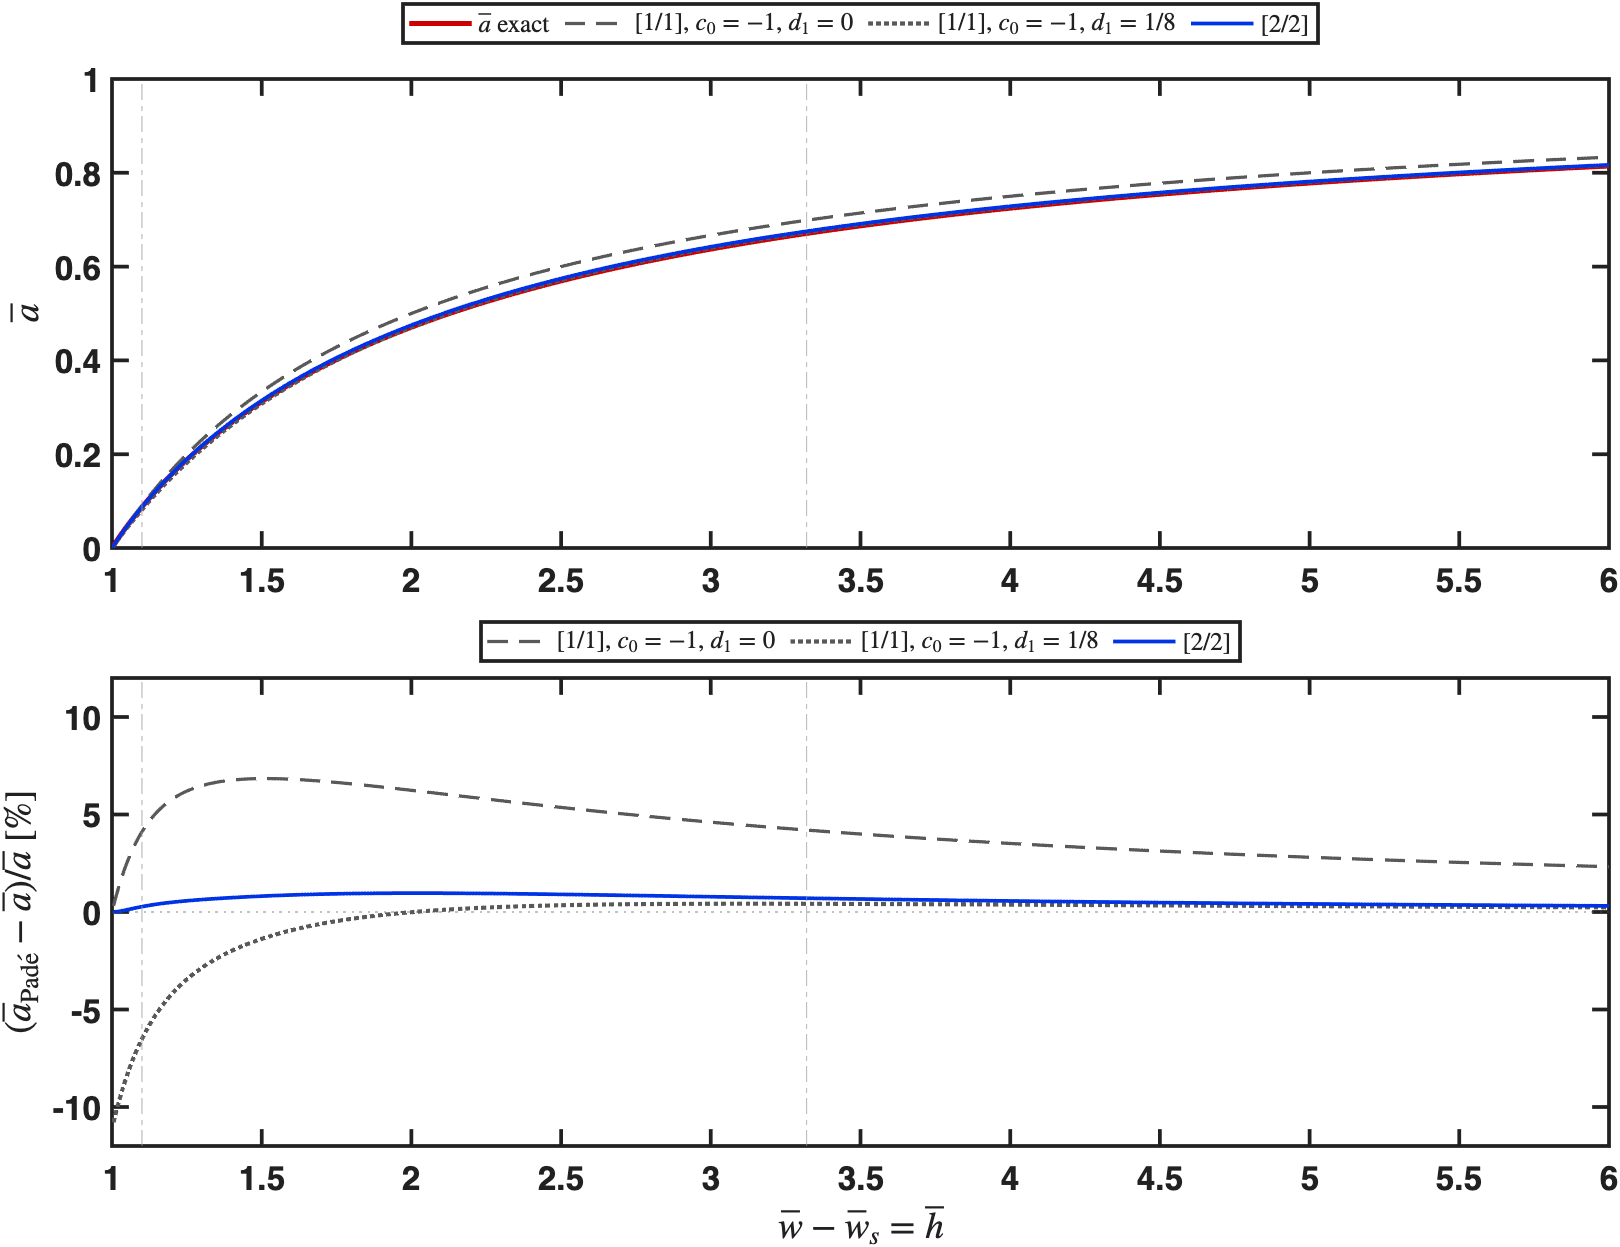
\includegraphics[width=\textwidth]{figures/plane_pade.png}

\newpage
\section{Two-point Pad\'e form of the cell (Fig.\ 11), $\bw_s$ = visible cell surface}

($\ba_z(\infty) = 1$ built in; $\bw_s$ is the visible surface, the zero of the Fig.\ 11 axis; coefficients by least squares on the
digitised curve over $1.1 \le \bw - \bw_s \le 5.5$ and the form is used there only; $\bw - \bw_s = 1$ lies outside the band;
the gain of the form vanishes at $\bw - \bw_s = -c_0$)

\begin{align*}
&[1/1] \\
\ba_z\gs
  &= \frac{\gs + c_0}{\gs + d_1} \\
\ba_z(1) &= \frac{1 + c_0}{1 + d_1} \\
\lim_{\bw - \bw_s \to \infty} \gs\,\bigl(1 - \ba_z\bigr) &= d_1 - c_0 \\[4pt]
&c_0 = 0.056,\quad d_1 = 1.197,\quad d_1 - c_0 = 1.141 \\
&\ba_z(1) = 0.481,\quad \ba_z(1.1) = 0.503 \ \text{(band floor)},\quad \ba_z = 0 \ \text{at}\ \bw - \bw_s = -0.056
\end{align*}

\begin{align*}
&[2/2] \\
\ba_z\gs
  &= \frac{\gs^{2} + c_1\,\gs + c_0}
          {\gs^{2} + d_1\,\gs + d_2} \\
\ba_z(1) &= \frac{1 + c_1 + c_0}{1 + d_1 + d_2} \\
\lim_{\bw - \bw_s \to \infty} \gs\,\bigl(1 - \ba_z\bigr) &= d_1 - c_1 \\[4pt]
&c_0 = 0.353,\quad c_1 = -0.571,\quad d_1 = 0.484,\quad d_2 = 0.058 \\
&\ba_z(1) = 0.507,\quad d_1 - c_1 = 1.055
\end{align*}

\begin{align*}
&\text{same law in the 2026-09-16 coordinate } \bw_s' = \bw_s + 1 \ (\text{variable } \bw - \bw_s' = \gs - 1): \\
[1/1]:\qquad c_0' &= c_0 + 1, \qquad d_1' = d_1 + 1 \\
[2/2]:\qquad c_0' &= c_0 + c_1 + 1, \qquad c_1' = c_1 + 2, \qquad d_1' = d_1 + 2, \qquad d_2' = d_2 + d_1 + 1
\end{align*}

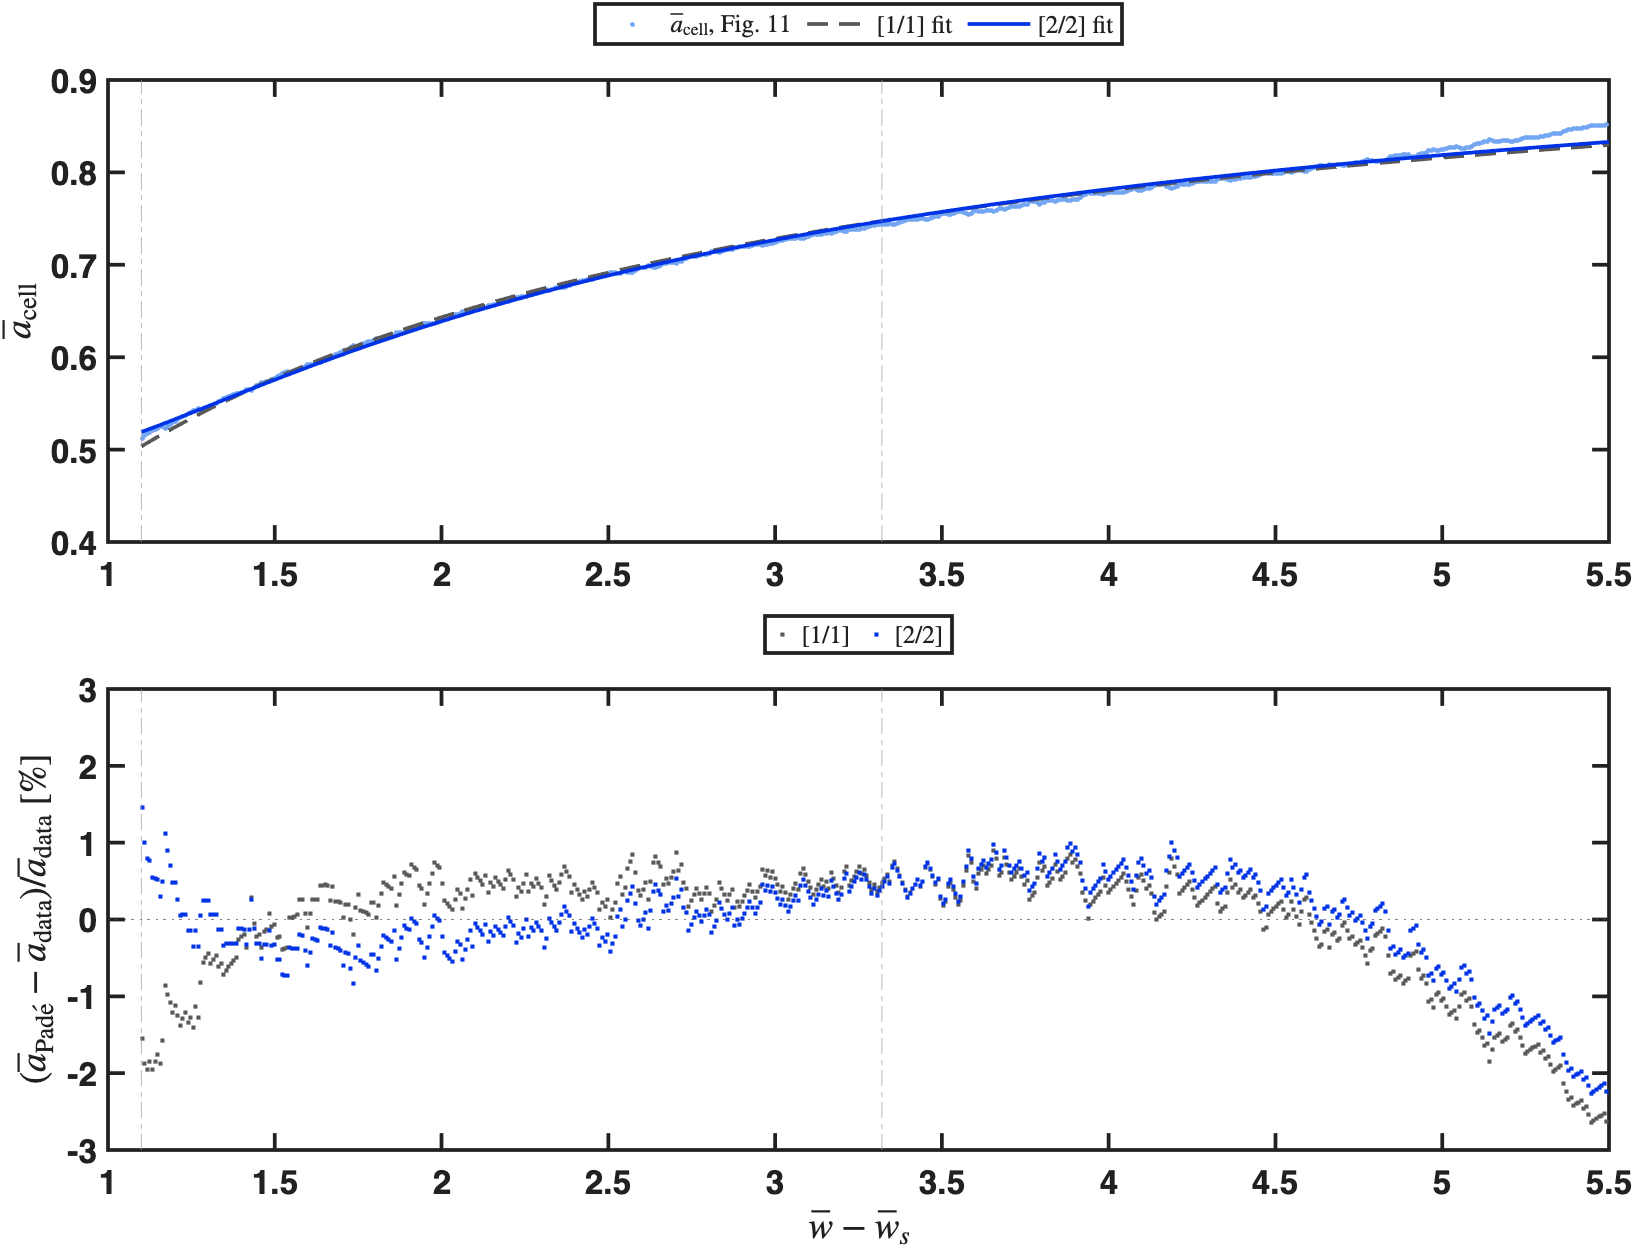
\includegraphics[width=\textwidth]{figures/cell_pade.png}

\end{document}
